\documentclass[11pt,a4paper]{article}

\usepackage[margin=0.92in]{geometry}
\usepackage[T1]{fontenc}
\usepackage[utf8]{inputenc}
\usepackage{lmodern}
\usepackage{microtype}
\usepackage{amsmath,amssymb,amsthm,mathtools}
\usepackage{booktabs}
\usepackage{array}
\usepackage{graphicx}
\usepackage{caption}
\usepackage{setspace}
\usepackage{enumitem}
\usepackage{tikz}
\usetikzlibrary{arrows.meta,positioning}
\usepackage{algorithm}
\usepackage{algpseudocode}
\usepackage{placeins}
\usepackage[authoryear,round]{natbib}
\usepackage[hidelinks]{hyperref}

\setstretch{1.035}
\setlist[itemize]{leftmargin=1.15em,itemsep=0.18em,topsep=0.3em}
\captionsetup{font=small,labelfont=bf,skip=6pt}
\captionsetup[figure]{name=Fig.,labelsep=space}
\setlength{\textfloatsep}{10pt plus 2pt minus 2pt}
\setlength{\floatsep}{8pt plus 2pt minus 2pt}
\setlength{\intextsep}{8pt plus 2pt minus 2pt}
\setlength{\abovecaptionskip}{6pt}
\setlength{\belowcaptionskip}{2pt}

\newtheorem{proposition}{Proposition}
\newtheorem{theorem}{Theorem}
\theoremstyle{definition}
\newtheorem{definition}{Definition}

\newcommand{\R}{\mathbb{R}}
\newcommand{\E}{\mathbb{E}}
\newcommand{\Prob}{\mathbb{P}}
\newcommand{\cF}{\mathcal{F}}
\newcommand{\1}{\mathbf{1}}

\title{\textbf{Anytime-Valid Typed Shift Monitoring with Covariate, Label, and Concept Witnesses under Sparse Labels}}
\author{%
Asher Mehfooz\\[1pt]
{\normalsize Department of Data Science, University of Kotli,}\\[-1pt]
{\normalsize Azad Jammu and Kashmir, Pakistan}
\and
Atif Ali\\[1pt]
{\normalsize Malaysian Institute of Information Technology, Universiti Kuala Lumpur}\\[-1pt]
{\normalsize (UniKL MIIT), 1016 Jalan Sultan Ismail, 50250 Kuala Lumpur, Malaysia}
}
\date{\small Corresponding author: Atif Ali, \texttt{dralexaly@gmail.com}}
\newcommand{\targetjournal}{Machine Learning (Springer Nature)}

\emergencystretch=2em
\begin{document}
\maketitle
\thispagestyle{empty}

\begin{abstract}
\noindent
Post-deployment distribution shift may reflect changes in the input marginal, class prevalence, or the conditional label mechanism, while continuous monitoring must control false alarms under data-dependent stopping. We propose Typed Shift Sequential Diagnosis (TSSD), an anytime-valid monitoring architecture for a frozen probabilistic classifier with sparse labels. TSSD maintains covariate, label, and concept witnesses built from bounded target--source paired increments. A predictable gate prevents the label process from accumulating evidence after strong covariate evidence, and fixed capital-mixture e-processes yield family-wise anytime-valid false-alarm control.

On 200 Gaussian null streams at $\alpha=0.05$, 3 alarm (1.5\%). In 200-stream primary experiments with 5\% label reveal, TSSD detects 200/200 covariate, 170/200 label, and 127/200 concept shifts after excluding pre-change alarms; 199, 170, and 127 are correctly singleton-typed. A power-optimized but still fixed two-sided concept bet improves concept detection without adding crossings on null, pure-covariate, or pure-label streams. Concept-witness power rises to 198/200 at 10\% label reveal, exposing the information bottleneck at 5\%. External BBSD-soft, classifier-CUSUM, Page--Hinkley, and a Roschewitz-style identification pipeline provide complementary comparisons. A 64-feature Digits benchmark and a chronological Mauna Loa CO$_2$ case study extend evaluation beyond controlled Gaussian streams. TSSD is therefore supported as a validity-preserving typed monitoring framework rather than a universally most-powerful detector.
\end{abstract}

\vspace{0.4em}
\noindent\textbf{Keywords:} dataset shift; sequential monitoring; e-process; anytime-valid inference; label shift; sparse labels.

\section{Introduction}
\label{sec:intro}

Post-deployment distribution shift is not a single failure mode. A frozen classifier may face a change in the input marginal, a change in class prevalence, or a change in the conditional relation between inputs and labels. These cases are usually described as covariate, label (or prior), and concept shift, respectively \cite{quinonero2009,moreno2012,gama2014,lu2019}. They also motivate different operational responses. A prior correction can be appropriate under label shift but inappropriate after the meaning of a label has changed; retraining or abstention may be more defensible under concept shift; and a benign covariate change need not justify either response. A sequential monitor should therefore do more than declare that ``something changed'': it should expose which source of evidence crossed, while retaining control of false alarms under continuous monitoring.

This problem is harder when labels are sparse. Unlabeled inputs provide immediate information about changes in the input distribution but cannot, by themselves, distinguish every shift mechanism. Conversely, a diagnostic that depends on a label at every time point is poorly matched to deployments in which only a small random fraction of outcomes are eventually observed. The setting studied here therefore combines an always-available input witness with label- and concept-oriented witnesses that exploit revealed outcomes when they exist.

We introduce Typed Shift Sequential Diagnosis (TSSD), an anytime-valid monitoring construction for a frozen probabilistic classifier. At each time point, every active witness compares the current target case with one independent source-reference case through the same score computed from predictable state. Clipping makes the resulting paired increment bounded. All three witnesses are converted to nonnegative capital-mixture e-processes. The label process is additionally controlled by a predictable gate: it may update only when the maximum covariate evidence available before the current pair is below a fixed log-evidence level. This design prevents a clear covariate departure from subsequently generating a spurious label diagnosis while preserving validity because the gate is measurable with respect to the past. Splitting a global false-alarm budget across the three witness e-processes gives family-wise anytime-valid control by Ville's inequality and a union bound. Unlike a fixed end-of-stream classifier, the diagnostic state is operational: it is the set of witnesses that have crossed by the current time and can therefore evolve after the initial alarm.

The empirical contribution is deliberately separated from the validity claim. The theorem controls false alarms under the stated global null; it does not guarantee high power against every alternative. We evaluate the revised monitor on a 200-replicate controlled study of each primary shift type, on a 64-feature handwritten-digits benchmark with controlled acquisition, prevalence, and concept changes, on a chronological Mauna Loa CO$_2$ monitoring case study, and against external detectors operating on the same streams. The revised label construction materially changes the earlier power picture: at 5\% label reveal it detects 170/200 pure label shifts while preserving 199/200 correct singleton covariate diagnoses. The external comparison is used to characterize complementary strengths rather than to claim universal state-of-the-art power.

The contributions are sixfold. First, TSSD provides three source-referenced, bounded sequential witnesses that share one online monitoring interface while preserving a global anytime-valid false-alarm level. Second, a predictably gated label capital process substantially improves scarce-label power without allowing later covariate evidence to contaminate the label process. Third, the paper proves the process property directly for the implemented witnesses, including the predictable gate. Fourth, the concept witness uses a fixed two-sided $\lambda=1$ capital bet, selected before the final confirmatory rerun, which improves scarce-label concept power while preserving the same martingale argument. Fifth, a 200-replicate evaluation, three established detector families, a higher-dimensional Digits benchmark, a Roschewitz-style identification comparison, and a chronological Mauna Loa CO$_2$ case study separate inferential validity from raw detection power. Sixth, the released package contains all calibration, null, shifted-stream, external-baseline, Digits, temporal-case, and figure-generation code required to regenerate the reported results.

\section{Related work and positioning}
\label{sec:related}

Dataset-shift taxonomies distinguish changes in the input marginal, class prevalence, and conditional labeling mechanism \cite{quinonero2009,moreno2012}; concept-drift surveys additionally study adaptation after such changes \cite{gama2014,lu2019}. TSSD is a monitoring method rather than an adaptation algorithm: the deployed classifier is frozen and the monitor accumulates evidence about departures from its source regime.

For input-distribution change, maximum mean discrepancy (MMD) is a standard kernel two-sample statistic \cite{gretton2012}. Rabanser et al. systematically compare dataset-shift detectors and introduce black-box shift detection (BBSD), which applies two-sample testing to a trained classifier's outputs \cite{rabanser2019}. We therefore include a BBSD-soft comparator that monitors class-probability outputs in fixed target blocks. The raw MMD-style contrast used as an ablation in this paper is intentionally simpler than TSSD's covariate witness. TSSD orthogonalizes the kernel score with respect to directions induced by the frozen classifier's class-probability vector, because a change in class prevalence can also change the marginal distribution of inputs.

Label shift is usually handled by estimating a new class prior while keeping class-conditional feature laws fixed. Expectation-maximization correction \cite{saerens2002}, black-box shift estimation \cite{lipton2018}, and unified treatments of label-shift estimation \cite{garg2020} provide the estimation background used by TSSD's label-oriented state. Evans and G'Sell study sequential label-shift detection directly and evaluate nonparametric changepoint procedures on simulated outbreaks based on real dengue data \cite{evans2024}. Their work is specialized to label shift and provides an important point of comparison for the weak label-witness power observed here.

Anytime-valid monitoring has a separate lineage. Nonnegative martingales and e-processes support inference under optional stopping \cite{ville1939,howard2020,vovk2021,ramdas2023,waudbysmith2024}. Vovk's online concept-shift note is especially close conceptually: conformal exchangeability martingales are decomposed into components associated with concept and label shift \cite{vovk2020concept}. Classical sequential change detection provides a different comparator: Page--Hinkley accumulates persistent deviations of an observed loss or signal from its running level \cite{page1954}. TSSD differs in using fresh source-reference pairing, explicit bounded score differences, a separate orthogonalized covariate witness, and a family-wise budget across three named witnesses under sparse random label reveal.

Recent deployment-monitoring work makes the novelty boundary narrower and must be stated explicitly. WATCH introduces weighted conformal test martingales that adapt to mild covariate shift and diagnose harmful changes as concept shift or extreme covariate shift, with real-world evaluations and state-of-the-art comparisons \cite{prinster2025watch}. M-FISHER uses a martingale-driven detector together with Fisher-preconditioned test-time adaptation and provides an anytime-valid detection analysis for covariate shift \cite{khan2025mfisher}. These methods are stronger than TSSD in dimensions that this paper does not claim to dominate, including adaptation and breadth of real-world evaluation. TSSD instead targets an interpretable three-witness decomposition with a single family-wise false-alarm budget and explicit use of sparse labels.

A complementary line of work identifies shift type without sequential anytime-valid guarantees. Roschewitz et al. distinguish prevalence, covariate, and mixed shifts across multiple medical-imaging datasets \cite{roschewitz2025}. Their study demonstrates why root-cause identification matters in practice. Relative to that setting, TSSD adds an online stopping rule and a concept witness, but its empirical study is substantially smaller. Accordingly, this paper does not claim state-of-the-art detection delay against WATCH, Evans--G'Sell, or Roschewitz et al. The contribution is the validity-preserving typed-witness construction and the evidence, including negative results, obtained from its released implementation.

\begin{table}[t]
\centering
\caption{Positioning against the closest lines of work. The entries summarize statistical scope rather than claim an empirical ranking across incompatible benchmarks.}
\label{tab:position}
\small
\begin{tabular}{@{}>{\raggedright\arraybackslash}p{0.16\textwidth}>{\raggedright\arraybackslash}p{0.22\textwidth}>{\raggedright\arraybackslash}p{0.22\textwidth}>{\raggedright\arraybackslash}p{0.31\textwidth}@{}}
\toprule
Method & Sequential object & Shift types emphasized & Distinction relative to TSSD \\
\midrule
Evans--G'Sell \cite{evans2024} & Classifier-score changepoint statistic & Label shift & Purpose-built label-shift detector; TSSD instead allocates one anytime-valid budget across three witnesses. \\
Vovk \cite{vovk2020concept} & Exchangeability martingales & Concept and label shift & Closest martingale decomposition; TSSD adds a separate source-referenced covariate witness and sparse-label interface. \\
WATCH \cite{prinster2025watch} & Weighted conformal martingales & Mild/extreme covariate and concept shift & Adds online adaptation and broader real-world evaluation; TSSD targets an explicit covariate/label/concept witness set. \\
Roschewitz et al. \cite{roschewitz2025} & Dataset-level detection and identification & Prevalence, covariate, and mixed shift & Strong empirical shift identification; TSSD adds an anytime-valid online stopping construction and a concept witness. \\
TSSD & Paired bounded e-processes & Covariate, label, and concept witnesses & Family-wise anytime-valid alarm with an online active-witness state under sparse random label reveal. \\
\bottomrule
\end{tabular}
\end{table}

\section{Problem formulation}
\label{sec:problem}

Let the source law be \(P\), with class prior \(\pi\) on \(\{1,\ldots,K\}\) and class-conditional input laws for \(X\in\R^d\). A source model \(g\) is fit on a sample from \(P\) and then frozen. It returns a probability vector \(p_g(x)\in\R^K\). At monitoring step \(t=1,\ldots,T\) the operator sees a target input \(x_t\), a reveal bit \(R_t\in\{0,1\}\), and a label \(y_t\) when \(R_t=1\). In the experiments \(R_t\) is drawn independently with \(\Prob(R_t=1)=\rho\), and \(\rho\) is either \(0.05\) or \(0.20\).

The monitor also receives one fresh source reference \((x'_t,y'_t)\sim P\), drawn independently of the target case and used at this step only. A stored source pool would play the same role in a deployment. The reference is not a second target case.

Write \(\cF_{t-1}\) for the history available before the current target and reference are scored: past target cases, past references, past reveal bits, and every estimate computed from them. A score used at time \(t\) has to be \(\cF_{t-1}\)-measurable. Estimates that depend on \((x_t,y_t)\) are stored for step \(t+1\), after the bet.

\begin{definition}[Online diagnostic state]
\label{def:names}
Let $\tau_X,\tau_L,\tau_C$ be the first crossing times of the covariate, label, and concept witnesses, with $\tau_k=\infty$ when witness $k$ has not crossed. Define the active set at time $t$ as
\[
\mathcal{A}_t=\{k\in\{X,L,C\}:\tau_k\le t\}.
\]
The alarm time is $\tau=\min_k\tau_k$. At any current time $t$, the diagnostic state is \emph{no evidence} if $\mathcal{A}_t$ is empty; covariate, label, or concept when $\mathcal{A}_t$ is the corresponding singleton; and \emph{multiple witnesses} when $|\mathcal{A}_t|\ge2$. Thus the state is available online and may be refined after the initial alarm. A horizon diagnostic reported in an experiment is simply the state at the prespecified terminal time $T$; it is not part of the monitoring rule and does not use an unknown future stopping point.
\end{definition}

The three pure alternatives used in the shift study are the usual ones. Covariate shift changes the marginal of \(X\) and keeps the conditional law of \(Y\) given \(X\). Label shift changes \(\pi\) and keeps the class-conditional input laws. Concept shift keeps the marginal of \(X\) and changes the conditional law of \(Y\) given \(X\). Section~\ref{sec:protocol} writes the generators actually sampled so that the names in the tables refer to those generators and not to a looser description.

The operating target under the global null is a false-alarm level \(\alpha\). Each witness is given \(\alpha_k=\alpha/3\). An alarm is the event that any witness ever crosses. Theorem~\ref{thm:validity} establishes that this event has probability at most \(\alpha\) when the target cases are still drawn from \(P\) under its stated assumptions. The experiments estimate that probability on a finite horizon. They do not estimate power by a theorem.

\section{The three witnesses}
\label{sec:witness}

The constants below are fixed before the reported controlled streams are evaluated. Covariate and concept capital bets use $\Lambda_C=\{0.5,1\}$. The label witness uses the fixed capital grid $\Lambda_L=\{0.01,0.05,0.10,0.25,0.50,1\}$. Both grids and the covariate gate $g_X=2$ on past maximum log-evidence were fixed before the reported streams were evaluated. Let the clip constants be
\begin{equation}
c_X=0.030549503301877223,\quad
c_L=0.30610870092768355,\quad
c_C=1.101259429554347.
\label{eq:clips}
\end{equation}
All three witness clips are reproduced by \texttt{code/calibrate\_clips.py}. Using source-only calibration seeds 9000--9019, disjoint from every reported null and shift stream, the script pools the absolute raw target and reference scores and takes their empirical 95th percentile. The resulting sample sizes are 16,000 raw scores for the covariate and label witnesses and 612 active raw concept scores. None of the clips is recomputed on a monitored stream. The raw-kernel MMD-e baseline is calibrated independently by the same rule, giving \(c_{\mathrm{MMD}}=0.05851293885375384\); this avoids imposing the orthogonalized covariate score's scale on the raw baseline. For a raw scalar \(u\) the clipped score is
\begin{equation}
s(u,c)=\mathrm{clip}(u,-c,c)/c\in[-1,1].
\label{eq:clip}
\end{equation}
If \(s_t\) is the clipped score of the target and \(s'_t\) is the clipped score of the fresh source reference, the increment is
\begin{equation}
D_t=\mathrm{clip}\big((s_t-s'_t)/2,\,-1,\,1\big)\in[-1,1].
\label{eq:D}
\end{equation}
The same formula produces \(D^X_t\), \(D^L_t\), and \(D^C_t\).

\subsection{Covariate witness}

The source fitting sample has \(n_0=2000\) labeled pairs. The Gaussian kernel width \(\sigma\) is the median pairwise Euclidean distance on those inputs. In this fit, \(\sigma=5.374491751357635\). The kernel is
\begin{equation}
k(a,b)=\exp\big(-\|a-b\|^2/(2\sigma^2)\big).
\label{eq:kernel}
\end{equation}
At step \(t\ge 2\), let \(W_t\) be the previous target inputs in a window of length at most 50, and let \(W'_t\) be the previous reference inputs in the same window. Both windows are known at time \(t-1\). The raw kernel contrast of a point \(x\) is
\begin{equation}
h_t(x)=\frac{1}{|W_t|}\sum_{u\in W_t}k(x,u)
-\frac{1}{|W'_t|}\sum_{u\in W'_t}k(x,u).
\label{eq:hraw}
\end{equation}
At \(t=1\) there is no past window, and both raw covariate scores are set to 0.

The source model supplies a \((K-1)\)-vector \(v(x)\), with entries \(p_g(x)_j/\pi_j-1\) for \(j=1,\ldots,K-1\). On the fitting sample these vectors form a matrix \(V_0\). The monitor freezes
\begin{equation}
G=\frac{1}{n_0}V_0^\top V_0+10^{-8}I_{K-1}
\label{eq:G}
\end{equation}
and uses a pseudoinverse of \(G\). A coefficient vector \(c_t\) and a scalar \(b_t\) are computed from the kernel means of the fitting sample against the current windows, exactly as in \texttt{covariate\_raw\_pair} in the released code. They do not depend on the current point. The orthogonalized score is
\begin{equation}
h^\perp_t(x)=h_t(x)-c_t^\top G^{-1}v(x)-b_t.
\label{eq:hperp}
\end{equation}
The target and the reference are each passed through \(h^\perp_t\), then through the clip \(c_X\), then through \eqref{eq:D}. Removing \(v(x)\) is the part of the witness that is supposed to ignore a pure change in class shares. The label-shift arm is the check of that choice.

\subsection{Label witness}

Let $q_{t-1}$ be the class-share estimate available before step $t$, with $q_0=\pi$. The estimate is kept in the restricted simplex $\{q:q_j\ge10^{-3},\sum_jq_j=1\}$ by the projection in the code. The raw label score of a probability vector $p$, a reveal bit $r$, and a label $y$ is
\begin{equation}
\ell(p,r,y,q)=
\begin{cases}
\log\big(\max\{(q/\pi)^\top p,10^{-8}\}\big), & r=0,\\[4pt]
\log\big(\max\{q_y/\pi_y,10^{-8}\}\big), & r=1.
\end{cases}
\label{eq:label}
\end{equation}
The target and reference are scored with the same reveal bit $R_t$; when $R_t=1$, each case uses its own label. The two raw scores are clipped with $c_L$ and combined by \eqref{eq:D}. Because $q_{t-1}$ is predictable and the fresh target/reference pair is exchangeable under the global null, $D_t^L$ is conditionally mean zero and bounded.

The revised process uses capital betting rather than a Hoeffding exponential. Let
\[
G_{t-1}^L=\mathbf 1\!\left\{\max_{s<t}\log E_s^X<g_X\right\},\qquad g_X=2.
\]
The gate is computed from covariate evidence available before the fresh pair at time $t$. If $G_{t-1}^L=1$, the label mixture is updated with factors $1\pm\lambda D_t^L$ for $\lambda\in\Lambda_L$; if the gate is closed, the label wealth is left exactly unchanged. Hence the gate cannot use the current target/reference increment to decide whether to bet. Empirically, this prevents a strong covariate departure from continuing to build label wealth while allowing label evidence to accumulate when the covariate witness remains quiet.

After the bet, $q$ is updated by ten Saerens-type EM steps. Unlabeled rows receive normalized weights proportional to $p_g(x)_j q_j/\pi_j$, while labeled rows add a count at the observed class. The result is projected back to the restricted simplex and stored as $q_t$; it is never used retrospectively inside $D_t^L$.

\subsection{Concept witness}

A shift in \(P(Y\mid X)\) need not look like an additive change in the logits. The concept arm in this paper cycles the label, which is a permutation of classes. An additive bias cannot represent a permutation, and it is exactly zero at the start. The concept witness is therefore a confusion matrix built only from labels revealed before the current step.

Let \(C_{t-1}\) be a \(K\times K\) matrix of counts. Rows are classes of the source model and columns are observed labels. It starts at \(C_0=\mathbf{1}\mathbf{1}^\top\), an add-one prior. On a labeled step, and only when at least five labels have already been stored, the raw concept score of a pair \((x,y)\) is
\begin{equation}
\begin{aligned}
R_{t-1}(y\mid k)&=C_{t-1}(k,y)\Big/\sum_{y'}C_{t-1}(k,y'),\\
a(y)&=\sum_{k=1}^{K}p_g(x)_k\,R_{t-1}(y\mid k),\\
\eta&\propto (q_{t-1}/\pi)\odot p_g(x),\\
\kappa&=\log\big(\max\{a(y),10^{-8}\}\big)-\log\big(\max\{\eta_y,10^{-8}\}\big).
\end{aligned}
\label{eq:concept}
\end{equation}
The vector \(\eta\) is normalized to sum to one. It is the label-shift adjustment. The matrix \(R_{t-1}\) is the concept adjustment. The same function is applied to the target pair and to the reference pair. Both raw values are clipped with \(c_C\) and combined by \eqref{eq:D}. The constant \(c_C\) is the 95th percentile of \(|\kappa|\) on source-only streams with seeds 9000 through 9019. Those seeds are not the streams in the tables.

If the step is unlabeled, or if fewer than five labels are already in hand, both concept scores are set to 0, so \(D^C_t=0\). The current label is not counted among those five. The first five revealed labels therefore contribute a zero concept increment.

The matrix is updated only after the bet, and only on a revealed label. Excess counts above the add-one prior are multiplied by \(0.85\), the prior is put back, and the source probability vector is added to the column of the observed label. The factor \(0.85\) lets labels from after a change outweigh labels from before it. Without that factor, a matrix fit on the whole past would stay close to the pre-change labeling for the rest of a horizon of 200 steps. The same matrix is used for the target and the reference, so under the null the two scores remain exchangeable.

Concept evidence is updated only when \(R_t=1\). An unlabeled step leaves the concept processes exactly where they were. A labeled step always updates them, including the early steps on which \(D^C_t=0\). On a capital bet that zero increment multiplies wealth by 1.

\section{Evidence, naming, and a proposed action}
\label{sec:evidence}

\subsection{Mixture e-process}

All three witnesses use capital mixtures. For a bounded mean-zero increment $D\in[-1,1]$ and $\lambda\in(0,1]$, the positive and negative components update as
\begin{equation}
\log M_t^{\lambda,+}=\log M_{t-1}^{\lambda,+}+\log(1+\lambda D),\qquad
\log M_t^{\lambda,-}=\log M_{t-1}^{\lambda,-}+\log(1-\lambda D).
\label{eq:bet}
\end{equation}
The covariate and concept witnesses use $\Lambda_C=\{0.5,1\}$; the label witness uses $\Lambda_L=\{0.01,0.05,0.10,0.25,0.50,1\}$. Each witness reports the equal arithmetic mixture of its positive and negative components. A zero increment or a predictably skipped update is an identity update and therefore leaves evidence unchanged.

A witness crosses at the first $t$ with
\begin{equation}
\log E_t\ge\log(1/\alpha_k)=\log(3/\alpha).
\label{eq:line}
\end{equation}
For $\alpha=0.05$ the line is $\log60=4.09434456222$. Covariate evidence updates at every step. Concept evidence updates only on revealed-label steps. Label evidence updates only while its predictable covariate gate is open. All mixtures are computed in log space using log-sum-exp.

\subsection{Alarm and diagnostic state}

The crossing times and online active set are those in Definition~\ref{def:names}. The family-wise alarm occurs at the first crossing, while the diagnostic state can later acquire additional witnesses without spending a second false-alarm budget. This distinction removes any dependence on an ``end of stream'' that a deployment would not know in advance.

For the controlled shift study, the change begins at 1-based step 201. A \emph{pre-change alarm} is any TSSD crossing before step 201. Such a stream has already alarmed operationally and is therefore not recycled, using knowledge of the simulated change point, as a later post-change success. A \emph{post-change detection} is counted only when no pre-change TSSD alarm occurred and the first TSSD crossing is at step 201 or later. Its delay is the crossing step minus 201. For descriptive diagnosis we report the active set at the fixed horizon $T=400$ only for streams without a pre-change alarm. This horizon diagnostic is a retrospective evaluation summary of the online state, not a rule used by the monitor.

\subsection{What the experiments do not score}
\label{sec:action}

A diagnostic state suggests an action, but this paper does not prove that any action controls excess risk. On every revealed label after the simulated change, the code records the log loss of three predictors formed from information available before that label: the frozen source probability \(p_g\), the label-shift adjustment \(\eta\) in \eqref{eq:concept}, and the concept adjustment \(a\). It also records an illustrative online policy driven by the current active set: use \(p_g\) when no witness or only the covariate witness is active, use \(\eta\) when only the label witness is active, use \(a\) when only the concept witness is active, and abstain when two or more witnesses are active. Importantly, pre-change crossings are not erased from this operational policy.

When the policy abstains, its log loss is undefined on that case. The reported policy loss is therefore a \emph{selective risk} computed only on covered labels and must be read together with coverage (one minus the abstention fraction). It is not directly comparable to a full-coverage predictor without an abstention cost, and no such cost is chosen here. None of the action columns is an anytime-valid risk guarantee.

Algorithm~\ref{alg:tssd} is one monitoring step in the order executed by the code.

\begin{algorithm}[t]
\caption{One TSSD step. State used in the scores is from before time \(t\).}
\label{alg:tssd}
\begin{algorithmic}[1]
\Require History \(\cF_{t-1}\), target \((x_t,R_t,y_t)\), fresh source pair \((x'_t,y'_t)\)
\State Read \(q_{t-1}\), \(C_{t-1}\), the kernel windows, and the processes of each witness
\State Form \(h^\perp_t(x_t)\) and \(h^\perp_t(x'_t)\); clip by \(c_X\); set \(D^X_t\) by \eqref{eq:D}
\State Form the label scores \eqref{eq:label} at \(R_t\); clip by \(c_L\); set \(D^L_t\)
\If{\(R_t=1\) and at least five labels are already stored}
  \State Form the concept scores \eqref{eq:concept}; clip by \(c_C\); set \(D^C_t\)
\Else
  \State Set \(D^C_t\gets 0\)
\EndIf
\State Record whether the label gate is open from past covariate evidence; update the covariate capital mixture
\If{the predictable label gate is open}
  \State Update the label capital mixture
\Else
  \State Leave the label mixture unchanged
\EndIf
\If{\(R_t=1\)}
  \State Update the concept capital mixture with \(D^C_t\)
\Else
  \State Leave the concept mixture unchanged
\EndIf
\State Cross any witness whose log-evidence is at least \(\log(1/\alpha_k)\); update the online active set
\State Append the current target probability to the EM history and recompute \(q_t\)
\If{\(R_t=1\)}
  \State Append the label and update \(C_t\) with decay \(0.85\)
\EndIf
\end{algorithmic}
\end{algorithm}

\section{Anytime-valid false-alarm control}
\label{sec:validity}

The guarantee below is for the global null that the monitored target cases continue to follow the same source law as the reference cases. It is a false-alarm theorem, not a power or identification theorem.

\begin{theorem}[Family-wise anytime-valid false-alarm control]
\label{thm:validity}
Fix $\alpha\in(0,1)$ and allocate $\alpha_X=\alpha_L=\alpha_C=\alpha/3$. Suppose that under the global null, conditional on $\mathcal F_{t-1}$, the target pair $Z_t=(X_t,Y_t)$ and source-reference pair $Z'_t=(X'_t,Y'_t)$ are independent draws from the same law $P$. Suppose $R_t$ is independent of $(Z_t,Z'_t)$ conditional on $\mathcal F_{t-1}$, and every state used to score or gate the current pair---including $q_{t-1}$, $C_{t-1}$, kernel windows, source-fit quantities, clip constants, and the label-gate indicator---is fixed before $(Z_t,Z'_t)$ is scored. Then all three implemented witness mixtures are nonnegative martingales starting at one, with identity updates on skipped concept or label-gate steps. Consequently,
\begin{equation}
\Pr\!\left(\exists t:\max_{k\in\{X,L,C\}}E_t^k\ge \frac{3}{\alpha}\right)\le\alpha.
\label{eq:level}
\end{equation}
Thus the first TSSD alarm is valid under optional stopping with no additional correction over time.
\end{theorem}

\begin{proof}
Condition on $\mathcal G_t=\sigma(\mathcal F_{t-1},R_t)$. For each active witness, the target and reference are passed through the same $\mathcal G_t$-measurable scoring function. Under the null, $(Z_t,Z'_t)$ is exchangeable given $\mathcal G_t$. Swapping the two cases changes the sign of the paired score difference in \eqref{eq:D}; because the outer clipping is odd, $D_t^k$ has a conditionally symmetric distribution, so $\mathbb E[D_t^k\mid\mathcal G_t]=0$ and $|D_t^k|\le1$.

For any capital component with $\lambda\in(0,1]$, nonnegativity follows from boundedness and
$\mathbb E[1\pm\lambda D_t^k\mid\mathcal G_t]=1$. Hence each positive- and negative-sign product is a nonnegative martingale, and so is any fixed finite arithmetic mixture. The concept witness uses an identity update on unlabeled steps. The revised label witness uses an identity update whenever $G_{t-1}^L=0$; because $G_{t-1}^L$ is $\mathcal F_{t-1}$-measurable, predictable skipping also preserves the martingale property. Ville's inequality gives $\Pr(\sup_t E_t^k\ge1/\alpha_k)\le\alpha_k$ for each witness, and a union bound across the three witnesses yields \eqref{eq:level}. Independence between witness processes is not required.
\end{proof}

The theorem depends on using a genuinely source-distributed reference at each step (or, conditional on a fixed empirical source pool, independent sampling from the same empirical law under the null) and on freezing calibration before monitoring. Re-estimating clip constants from future monitored observations would violate predictability. The theorem also does not imply that a crossing witness uniquely identifies an arbitrary alternative, does not provide a detection-delay bound, and does not control the risk of the illustrative action policy.

\section{Experimental protocol}
\label{sec:protocol}

\subsection{Controlled Gaussian benchmark}
The primary benchmark uses $K=3$, $d=10$, a uniform source prior, class-conditional $N(\mu_y,I_{10})$ inputs, and one frozen multinomial logistic-regression source model trained on 2000 source pairs. The class means are generated once with NumPy seed 0 and the model-fitting seed is 2026. Monitoring uses $T=400$ with a change at step 201, independent source-reference draws, and label reveal rate $\rho=0.05$. The witness clips are calibrated on disjoint source-only seeds 9000--9019 by the empirical 95th percentile of the absolute raw scores:
\[
c_X=0.030549503301877223,\quad c_L=0.30610870092768355,\quad c_C=1.101259429554347.
\]
The global alarm level is $\alpha=0.05$, so each witness crosses at $\log60$. Covariate capital rates are $\{0.5,1\}$; the concept witness uses the fixed two-sided rate $\lambda_C=1$; label capital rates are $\{0.01,0.05,0.10,0.25,0.50,1\}$ and the predictable covariate gate is $g_X=2$.

The three primary alternatives are deliberately interpretable. Covariate shift translates every class cloud by $(2,\ldots,2)$ while labels are redrawn from the original Bayes posterior. Label shift changes class shares to $(0.70,0.20,0.10)$ while preserving $P(X\mid Y)$. Concept shift preserves the source input mixture and cycles the observed class by one modulo 3. Each primary arm contains 200 streams. A stream with a TSSD crossing before step 201 is counted as a pre-change alarm and is not recycled as a post-change success.

\subsection{External detectors}
Three established detector families are evaluated on the same Gaussian streams. BBSD-soft applies classwise two-sample Kolmogorov--Smirnov statistics to 50-case blocks of classifier probabilities. A multiclass classifier-CUSUM adapts the sequential label-shift construction of Evans and G'Sell to a fixed grid of three-class alternative priors. Page--Hinkley is applied to revealed predictive log loss after at least five labels. Because these comparators do not share TSSD's family-wise anytime-valid guarantee, each threshold is calibrated to the empirical 95th percentile of its maximum statistic on 1000 disjoint source-only streams and checked on 1000 additional null streams. Each external shifted arm contains 200 streams.

\subsection{Higher-dimensional real-data stress test}
To move beyond Iris/Wine-scale examples, we use the scikit-learn handwritten Digits dataset (1797 real images represented by 64 intensity features and 10 classes) \citep{pedregosa2011}. A fixed stratified 60\% split fits the source classifier and the remaining 40\% supplies an empirical source pool. The horizon is 300, the change begins at step 151, and labels are revealed independently at 5\%. Source-only calibration uses ten disjoint streams; evaluation uses 50 null streams and 50 streams for each shift arm. Label shift oversamples classes 0--2 while preserving empirical $X\mid Y$; concept shift cycles the digit label; and the acquisition-shift arm applies a fixed contrast increase plus Gaussian sensor noise to the held-out real images. These are controlled changes on real 64-dimensional measurements, not claims of naturally occurring temporal drift.

We also implement the published identification logic of Roschewitz et al. \citep{roschewitz2025} on the same Digits batches: dual BBSD+MMD detection, prevalence estimation, prevalence-adjusted reference resampling, feature re-testing, and output re-testing to distinguish prevalence from covariate/mixed shift. Their original pipeline uses medical-image SSL encoders; the common Digits experiment substitutes the same 64-dimensional standardized image representation, so the comparison tests the identification logic rather than claiming a reproduction of the original medical feature extractor.

\section{Results}
\label{sec:results}

\subsection{Null control and primary 200-replicate study}
Table~\ref{tab:primary} reports the revised TSSD monitor. Under the global null, 3 of 200 streams alarm, an empirical rate of 1.5\% with Wilson 95\% interval $[0.51,4.32]\%$. This finite simulation is consistent with, but is not the basis of, the theorem-backed 5\% family-wise bound.

\begin{table}[t]
\centering
\caption{Revised TSSD primary study at 5\% label reveal. ``Correct'' is the expected singleton horizon state among valid post-change detections.}
\label{tab:primary}
\small
\begin{tabular}{lrrrr}
\toprule
Condition & Pre-change & Detected & Correct & Median delay \\
\midrule
Covariate & 0/200 & 200/200 & 199/200 & 43.0 \\
Label & 4/200 & 170/200 & 170/200 & 129.5 \\
Concept & 1/200 & 127/200 & 127/200 & 150.0 \\
\bottomrule
\end{tabular}
\end{table}

The principal change relative to the earlier label construction is substantial: pure label-shift detection rises from a low-power regime to 170/200 valid detections while covariate specificity is retained at 199/200 correct singleton states. The one multiple-witness covariate case is visible in the released CSV. Using the fixed $\lambda_C=1$ two-sided concept capital improves valid concept detections from 102/200 to 127/200 without adding a concept crossing on any of the 200 null, 200 pure-covariate, or 200 pure-label streams. The remaining gap is strongly label-budget driven: in independent concept-only sensitivity runs the concept witness crosses in 128/200 streams at 5\% reveal and 198/200 streams at both 10\% and 20\% reveal, with median post-change label counts of approximately 10, 19, and 39 respectively.

\subsection{Common-stream external comparison}
The horizon-calibrated external detectors behave as expected for their intended alternatives. On 1000 independent null-check streams, BBSD-soft, classifier-CUSUM, and Page--Hinkley each alarm in 55 streams. On the 200 shifted streams, BBSD-soft detects 194 covariate, 198 label, and 6 concept streams; classifier-CUSUM detects 197, 194, and 11; and Page--Hinkley detects 8, 3, and 198, respectively. TSSD therefore does not dominate specialized detectors in raw power. Its distinct contribution is simultaneous typed evidence with a formal family-wise anytime-valid guarantee.

\begin{figure}[t]
\centering
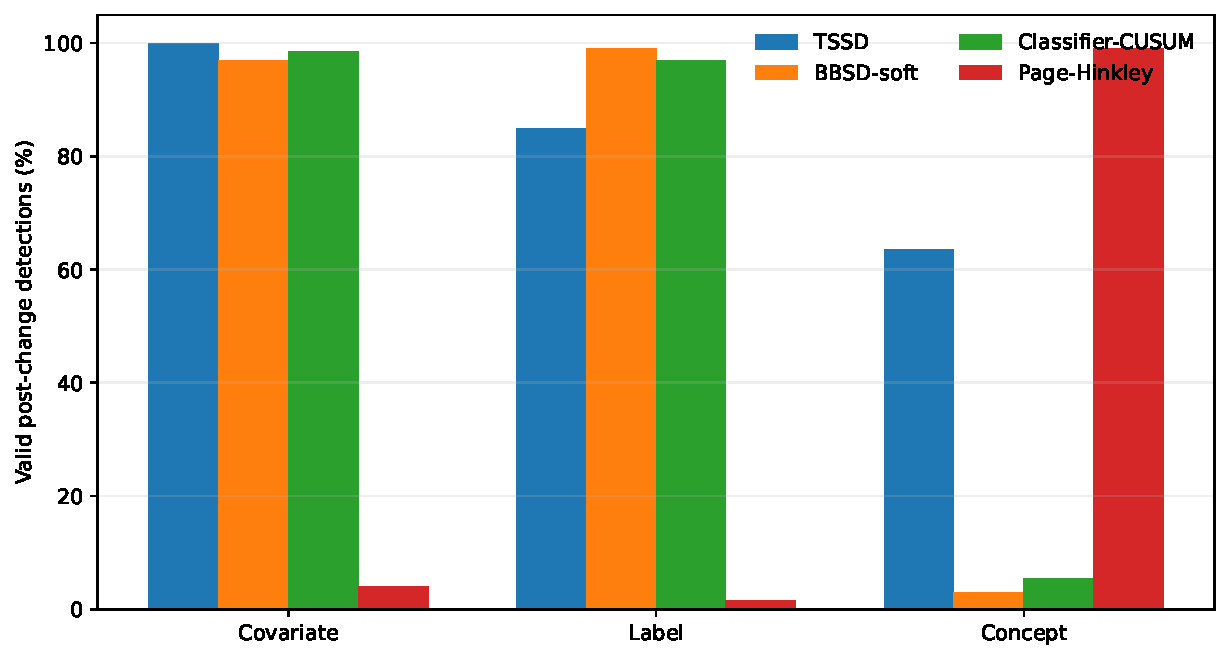
\includegraphics[width=0.86\textwidth]{Fig1.pdf}
\caption{Common-stream detection comparison on the 200-replicate Gaussian study. External thresholds are finite-horizon calibrated; TSSD uses the theorem-backed witness threshold.}
\label{fig:external}
\end{figure}

\subsection{Higher-dimensional Digits benchmark}
Table~\ref{tab:digits} gives the 64-feature Digits stress test. The revised monitor has one alarm among 50 null streams. The acquisition corruption is detected and correctly singleton-typed in all 50 streams. The deliberately strong prevalence shift is detected in 40/50 streams; 29 are label singletons and five are multiple-witness states, so the label component is active in 34/50 streams. Concept shift is detected and correctly typed in 21/50 streams at the short horizon and 5\% reveal rate. The result confirms that the revised label witness is not restricted to the Gaussian generator, although type separation remains representation- and horizon-dependent.

\begin{table}[t]
\centering
\caption{TSSD on the 64-feature handwritten-digits stress test.}
\label{tab:digits}
\small
\begin{tabular}{lrrrr}
\toprule
Condition & Pre-change & Detected & Correct singleton & Multiple \\
\midrule
Acquisition/covariate & 0/50 & 50/50 & 50 & 0 \\
Label/prevalence & 1/50 & 40/50 & 29 & 5 \\
Concept & 1/50 & 21/50 & 21 & 0 \\
\bottomrule
\end{tabular}
\end{table}

The Roschewitz-style identification pipeline alarms on 2/50 null batches and identifies 47/50 label-shift batches as prevalence shift. On the chosen acquisition corruption it detects all 50 batches but classifies them as prevalence rather than covariate after prevalence adjustment. This negative result is informative rather than hidden: the published logic is sensitive to the representation used for feature testing, and the raw standardized digit representation does not reproduce the medical-image SSL features for which that pipeline was designed. TSSD's acquisition witness, by contrast, correctly singles out all 50 of these streams.

\begin{table}[t]
\centering
\caption{Concept-witness label-budget sensitivity on 200 independent concept-shift streams. The 5\% row is the primary setting; the higher rates are prespecified sensitivity runs for the same fixed concept e-process.}
\label{tab:concept_sens}
\small
\begin{tabular}{lrr}
\toprule
Label reveal & Concept crossings & Median post-change labels \\
\midrule
5\% & 128/200 & 10 \\
10\% & 198/200 & 19 \\
20\% & 198/200 & 39 \\
\bottomrule
\end{tabular}
\end{table}

\subsection{Chronological real-data monitoring case study}
To add a genuinely time-indexed deployment-style check, we use the weekly Mauna Loa atmospheric CO$_2$ record distributed with statsmodels, covering March 1958--December 2001 \citep{keeling2004}. Weekly values are interpolated only at missing timestamps. A frozen logistic model predicts whether the following week's concentration will exceed the current week's value from ten lag, difference, moving-average, and seasonal features. The first 800 usable weeks fit the model, the next 400 form a fixed empirical source-reference pool, and the following 600 weeks (27 June 1981--19 December 1992) are monitored in chronological order. Reference cases are sampled independently with replacement from the fixed source pool and only 5\% of target labels are revealed to TSSD. Clip constants are calibrated on five source-only resampling streams before monitoring.

The real sequence produces a covariate-witness alarm at monitoring index 12 (19 September 1981), while neither the label nor concept witness crosses. This is consistent with the long-term evolution of the measured CO$_2$ process and should be interpreted as evidence of departure from the frozen early-period source distribution, not as ground-truth proof of a structural causal shift. As an offline contextual check using all available labels, frozen-model accuracy falls from 0.74 in the first 200 monitored weeks to 0.70 in the last 200, while log loss rises from 0.517 to 0.606. The case study therefore demonstrates chronological operation on a naturally evolving measured process without manufacturing a change point or a shift label.

\begin{table}[t]
\centering
\caption{Chronological Mauna Loa CO$_2$ case study (600 monitored weeks, 5\% label reveal).}
\label{tab:co2}
\small
\begin{tabular}{lr}
\toprule
Quantity & Result \\
\midrule
Monitoring period & 27 Jun 1981--19 Dec 1992 \\
Revealed labels & 19/600 \\
First TSSD witness crossing & Covariate, 19 Sep 1981 \\
Label / concept crossing & None / none \\
Frozen accuracy, first / last 200 & 0.74 / 0.70 \\
Frozen log loss, first / last 200 & 0.517 / 0.606 \\
\bottomrule
\end{tabular}
\end{table}

\subsection{Interpretation}
The experiments now support three narrower claims. First, the family-wise false-alarm statement is theoretical and survives the revised label gate because the gate is predictable. Second, scarce-label power is no longer dominated by a nonfunctional label witness: 170/200 Gaussian label streams are detected at 5\% label reveal, with strong covariate specificity. Third, no detector is uniformly best: output-distribution methods are strong for prevalence changes, loss monitoring is strong for concept changes, and representation choice materially affects covariate-versus-prevalence decomposition.

\section{Discussion and limitations}
\label{sec:discuss}

The revised label process addresses the largest weakness of the earlier manuscript. Replacing the conservative Hoeffding update with a bounded capital mixture increases label-shift power, while the predictable covariate gate prevents that more aggressive process from continuing to bet after strong covariate evidence has emerged. The primary study therefore moves from very low label power to 170/200 valid detections without sacrificing the main covariate result. The theorem changes correspondingly: all three witnesses are capital-mixture martingales, with predictable identity updates for the label gate and for unrevealed concept steps.

The remaining limitations are empirical rather than hidden inconsistencies. Concept power at 5\% reveal is still lower than covariate and label power, but the fixed $\lambda_C=1$ bet raises the valid primary result to 127/200 and the label-budget sensitivity reaches 198/200 at 10\% reveal. This pattern is consistent with an information bottleneck: only about ten post-change labels are expected in the 5\% Gaussian setting and fewer in the shorter Digits post-change segment. The Digits prevalence arm also shows that a label component can coexist with residual covariate evidence, so ``multiple witnesses'' should be read as accumulated evidence rather than a proof that two structural mechanisms truly changed. More generally, type separation depends on the quality of the frozen probabilistic representation and on how well its nuisance directions span prevalence-induced changes.

The modern comparison is intentionally careful. WATCH provides a different weighted-conformal monitoring and adaptation framework \citep{prinster2025watch}; reproducing its complete adaptation stack would change the task from typed shift identification to adaptive deployment monitoring. Roschewitz et al. provide a closer prevalence-versus-covariate identification pipeline \citep{roschewitz2025}; we implement its identification logic on a common Digits representation, but not its modality-specific medical SSL encoder. This is a stronger comparison than citation-only positioning, yet it should not be described as bit-for-bit reproduction of their medical experiments. The released code makes this adaptation explicit.

Digits remains a controlled stress test, but the added Mauna Loa case study removes the earlier controlled-only evaluation gap by running TSSD prospectively over a naturally ordered measured sequence with no manufactured change point. Because that case has no oracle shift-type labels, it is evidence of operational chronological monitoring rather than a power benchmark. Similarly, the theorem assumes fresh or conditionally independent source-reference sampling, a reveal process independent of the current target/reference pair, and calibration fixed before monitoring. Dependence, active label acquisition, or repeated use of a small reference archive would require a separate validity analysis.

Finally, the present work controls false alarms for shift evidence, not predictive risk after an alarm. Selecting an adaptation, retraining policy, or abstention rule requires additional guarantees. We therefore avoid claiming universal state-of-the-art detection or automatic mitigation.

\section{Conclusion}
\label{sec:conclusion}

TSSD combines covariate, label, and concept evidence under one family-wise anytime-valid monitoring budget. The final formulation uses source-referenced bounded capital mixtures for all three witnesses and a predictable covariate gate for the label process. This change materially improves scarce-label prevalence detection while preserving the null argument and covariate specificity: in the 200-stream primary study, TSSD detects 200/200 covariate, 170/200 label, and 127/200 concept shifts at 5\% label reveal, with 199, 170, and 127 correct singleton diagnoses respectively among the reported streams. Concept-witness sensitivity rises to 198/200 at 10\% label reveal, and the chronological CO$_2$ case study demonstrates deployment-style operation without an artificial change point.

External detectors remain stronger on some specialized alternatives, and the higher-dimensional Digits experiment shows both improved generality and continuing representation dependence. The appropriate claim is therefore not universal superiority, but an inferentially explicit architecture that supplies simultaneous typed evidence with theorem-backed time-uniform false-alarm control and reproducible empirical evaluation.

\appendix
\section{Reproducibility and submission materials}
\label{sec:files}

The archive contains the exact scripts and CSV outputs used in the revised manuscript: \path{code/run_no_shift.py} for the 200-stream null study; \path{code/run_shift_study.py} and \path{code/run_core200_one.py} for the primary 200-replicate shifts; \path{results/core200_results.csv} for the merged primary outputs; \path{code/run_external_baselines.py} for BBSD-soft, classifier-CUSUM, and Page--Hinkley; \path{code/run_digits_benchmark.py} for the 64-feature Digits stress test; \path{code/run_roschewitz_digits.py} for the Roschewitz-style identification comparison; and \path{code/run_co2_temporal.py} for the chronological Mauna Loa case study. Figure-generation scripts and all frozen thresholds are included in the same package.

\section*{Statements and Declarations}
\textbf{Competing interests.} A final author-attested competing-interest statement is required before submission; the reproducibility package includes an author sign-off checklist so that this declaration is not inferred or fabricated.\par
\textbf{Funding.} A final author-attested funding statement is required before submission; no funding claim is inferred from the computational package.\par
\textbf{Data availability.} The Gaussian benchmark is generated by the released scripts. The higher-dimensional experiment uses the public Digits dataset distributed with scikit-learn. The chronological case study uses the public Mauna Loa weekly atmospheric CO$_2$ dataset distributed with statsmodels. All derived CSV outputs used in the manuscript are included in the reproducibility archive.\par
\textbf{Code availability.} Complete executable source code for calibration, monitoring, external comparisons, and figure generation is included with the submission package.\par
\textbf{Author contributions.} Final CRediT roles require author attestation and are listed on the submission sign-off checklist.\par
\textbf{AI-assisted workflow disclosure.} ChatGPT (OpenAI; accessed October 2026) was used to assist with manuscript revision, code generation/debugging, and consistency checking. The executable scripts and saved outputs in the accompanying package provide the auditable computational record. The human authors remain responsible for verifying the final code, numerical results, citations, interpretations, and submitted text.\par

\begin{thebibliography}{99}
\bibitem[Evans and G'Sell(2024)]{evans2024}
C.~Evans and M.~G'Sell.
Sequential label shift detection in classification data: An application to dengue fever.
\textit{PLOS ONE}, 19(9):e0310194, 2024.

\bibitem[Gama et al.(2014)]{gama2014}
J.~Gama, I.~\v{Z}liobait\.{e}, A.~Bifet, M.~Pechenizkiy, and A.~Bouchachia.
A survey on concept drift adaptation.
\textit{ACM Computing Surveys}, 46(4), Article 44, 2014.

\bibitem[Garg et al.(2020)]{garg2020}
S.~Garg, Y.~Wu, S.~Balakrishnan, and Z.~C. Lipton.
A unified view of label shift estimation.
In \textit{Advances in Neural Information Processing Systems}, 2020.

\bibitem[Gretton et al.(2012)]{gretton2012}
A.~Gretton, K.~M. Borgwardt, M.~J. Rasch, B.~Sch\"olkopf, and A.~Smola.
A kernel two-sample test.
\textit{Journal of Machine Learning Research}, 13:723--773, 2012.

\bibitem[Howard et al.(2020)]{howard2020}
S.~R. Howard, A.~Ramdas, J.~McAuliffe, and J.~Sekhon.
Time-uniform Chernoff bounds via nonnegative supermartingales.
\textit{Probability Surveys}, 17:257--317, 2020.

\bibitem[Khan and Syed(2025)]{khan2025mfisher}
B.~Khan and T.~Q. Syed.
Technical note on sequential test-time adaptation via martingale-driven Fisher prompting.
\textit{arXiv preprint arXiv:2510.03839}, 2025; revised 2026.

\bibitem[Lipton et al.(2018)]{lipton2018}
Z.~C. Lipton, Y.-X. Wang, and A.~J. Smola.
Detecting and correcting for label shift with black box predictors.
In \textit{Proceedings of the 35th International Conference on Machine Learning}, PMLR 80, 2018.

\bibitem[Keeling and Whorf(2004)]{keeling2004}
C.~D. Keeling and T.~P. Whorf.
Atmospheric CO$_2$ concentrations derived from flask air samples at sites in the SIO network.
In \textit{Trends: A Compendium of Data on Global Change}. Carbon Dioxide Information Analysis Center, Oak Ridge National Laboratory, 2004.

\bibitem[Lu et al.(2019)]{lu2019}
J.~Lu, A.~Liu, F.~Dong, F.~Gu, J.~Gama, and G.~Zhang.
Learning under concept drift: A review.
\textit{IEEE Transactions on Knowledge and Data Engineering}, 31(12):2346--2363, 2019.

\bibitem[Moreno-Torres et al.(2012)]{moreno2012}
J.~G. Moreno-Torres, T.~Raeder, R.~Alaiz-Rodr\'iguez, N.~V. Chawla, and F.~Herrera.
A unifying view on dataset shift in classification.
\textit{Pattern Recognition}, 45(1):521--530, 2012.

\bibitem[Page(1954)]{page1954}
E.~S. Page.
Continuous inspection schemes.
\textit{Biometrika}, 41(1/2):100--115, 1954.

\bibitem[Pedregosa et al.(2011)]{pedregosa2011}
F.~Pedregosa et al.
Scikit-learn: Machine learning in Python.
\textit{Journal of Machine Learning Research}, 12:2825--2830, 2011.

\bibitem[Prinster et al.(2025)]{prinster2025watch}
D.~Prinster, X.~Han, A.~Liu, and S.~Saria.
WATCH: Adaptive monitoring for AI deployments via weighted-conformal martingales.
In \textit{Proceedings of the 42nd International Conference on Machine Learning}, PMLR 267:49830--49859, 2025.

\bibitem[Qui\~nonero-Candela et al.(2009)]{quinonero2009}
J.~Qui\~nonero-Candela, M.~Sugiyama, A.~Schwaighofer, and N.~D. Lawrence, editors.
\textit{Dataset Shift in Machine Learning}.
MIT Press, 2009.

\bibitem[Rabanser et al.(2019)]{rabanser2019}
S.~Rabanser, S.~G\"unnemann, and Z.~C. Lipton.
Failing loudly: An empirical study of methods for detecting dataset shift.
In \textit{Advances in Neural Information Processing Systems}, 2019.

\bibitem[Ramdas et al.(2023)]{ramdas2023}
A.~Ramdas, P.~Gr\"unwald, V.~Vovk, and G.~Shafer.
Game-theoretic statistics and safe anytime-valid inference.
\textit{Statistical Science}, 38(4):576--601, 2023.

\bibitem[Roschewitz et al.(2025)]{roschewitz2025}
M.~Roschewitz, R.~Mehta, C.~Jones, and B.~Glocker.
Automatic dataset shift identification to support safe deployment of medical imaging AI.
In \textit{Medical Image Computing and Computer Assisted Intervention -- MICCAI 2025}, LNCS 15966, pp.~67--76, 2025.

\bibitem[Saerens et al.(2002)]{saerens2002}
M.~Saerens, P.~Latinne, and C.~Decaestecker.
Adjusting the outputs of a classifier to new a priori probabilities: A simple procedure.
\textit{Neural Computation}, 14(1):21--41, 2002.

\bibitem[Ville(1939)]{ville1939}
J.~Ville.
\textit{\'Etude critique de la notion de collectif}.
Gauthier-Villars, 1939.

\bibitem[Vovk(2020)]{vovk2020concept}
V.~Vovk.
Testing for concept shift online.
\textit{arXiv preprint arXiv:2012.14246}, 2020.

\bibitem[Vovk and Wang(2021)]{vovk2021}
V.~Vovk and R.~Wang.
E-values: Calibration, combination, and applications.
\textit{The Annals of Statistics}, 49(3):1736--1754, 2021.

\bibitem[Waudby-Smith and Ramdas(2024)]{waudbysmith2024}
I.~Waudby-Smith and A.~Ramdas.
Estimating means of bounded random variables by betting.
\textit{Journal of the Royal Statistical Society: Series B}, 2024.
\end{thebibliography}

\end{document}
